% Preamble
\documentclass[12pt]{article}
\usepackage{graphicx}
\usepackage{listings} % For code listing
\usepackage{hyperref}

% Packages
\usepackage{amsmath}
\usepackage{amssymb}
\usepackage{amsthm}
\usepackage{geometry}
\usepackage{setspace}
\usepackage{xcolor}
\usepackage{enumitem}

% Custom colors for code highlighting
\definecolor{codegreen}{rgb}{0,0.6,0}
\definecolor{codegray}{rgb}{0.5,0.5,0.5}
\definecolor{codepurple}{rgb}{0.58,0,0.82}
\definecolor{backcolour}{rgb}{0.95,0.95,0.92}

% Style for code
\lstset{
    language=C,
    backgroundcolor=\color{backcolour},
    commentstyle=\color{codegreen},
    keywordstyle=\color{magenta},
    numberstyle=\tiny\color{codegray},
    stringstyle=\color{codepurple},
    basicstyle=\ttfamily\small,
    breakatwhitespace=false,
    breaklines=true,
    captionpos=b,
    keepspaces=true,
    numbers=left,
    numbersep=5pt,
    showspaces=false,
    showstringspaces=false,
    showtabs=false,
    tabsize=2
}

% Set up the page margins
\geometry{left=0.5in,right=0.5in,top=0.5in,bottom=0.75in}

% Document
\begin{document}

\title{Analysis of Forking Processes in a UNIX Environment}
\author{Abraham J. Reines}
\date{\today}

\maketitle

\begin{abstract}
This report explains the process of executing a program intended to demonstrate the forking of processes in a UNIX environment. Running a C program to create multiple processes using the forking command and system calls facilitated an undertanding of differences between on-screen and redirect output to files with and without the use of \texttt{fflush(stdout)}. The findings demonstrate the technicalities of process managemetn in concurrent systems. This draws attention to the use of buffer management for output behavior. 
\end{abstract}

\section{Introduction}
The process of forking is fundamental in UNIX and POSIX-compliant operating systems. This report aims to explore the behavior of the fork system call and its implications on process management and output buffering.

\section{Methodology}
The C program is compiled and executed on a UNIX system. The output is observed on-screen, redirected to a file, and appended to another file to analyze the behavior of process output under different conditions.

\section{Code Explanation}
The provided C program\footnote{See next page for the full code listing.} utilizes the \texttt{fork()} system call, which is fundamental for creating child processes in UNIX. When \texttt{fork()} is called, the current process is duplicated, creating a child process with a new process ID. The child process receives a copy of the parent's memory, but as execution continues, their states may diverge. The \texttt{getpid()} and \texttt{getppid()} functions retrieve the process ID and parent process ID, respectively, which are used in the output to track process lineage. The use of \texttt{fflush(stdout)} ensures that the standard output buffer is flushed immediately, affecting the order and visibility of the output across different processes.

\newpage
  \subsection{With fflush}
The use of fflush(stdout) ensures that the output buffer is flushed after each print statement, which affects how often the output is written to the terminal or file. *See next page for code. 

\lstinputlisting[language=C]{forking.c}

\subsection{Without fflush}
Commenting out the fflush(stdout) statement changes the program's behavior due to the output buffer not being manually flushed after each print statement.

\lstinputlisting[language=C]{forking_no_fflush.c}

\newpage
  \section{Results and Analysis}
This section will include the screenshots of the terminal output and the contents of the output files to illustrate the effects of forking and output buffering.

\subsection{Terminal Output with fflush}
\begin{figure}[h]
\centering
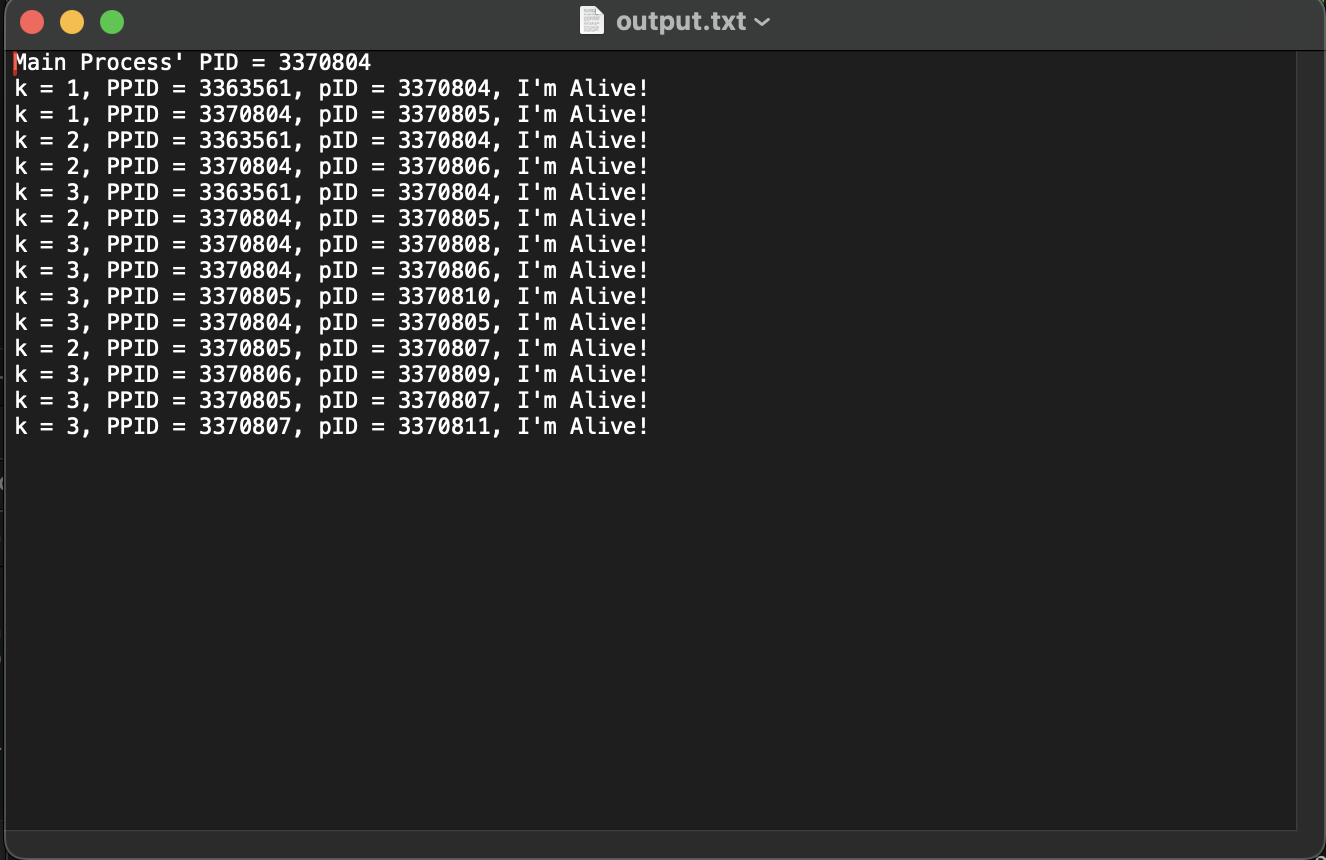
\includegraphics[width=\textwidth]{output_with_fflush.png}
\caption{Terminal output when fflush is used.}
\end{figure}

\newpage
  \subsection{Terminal Output without fflush}
  \begin{figure}[h]
    \centering
    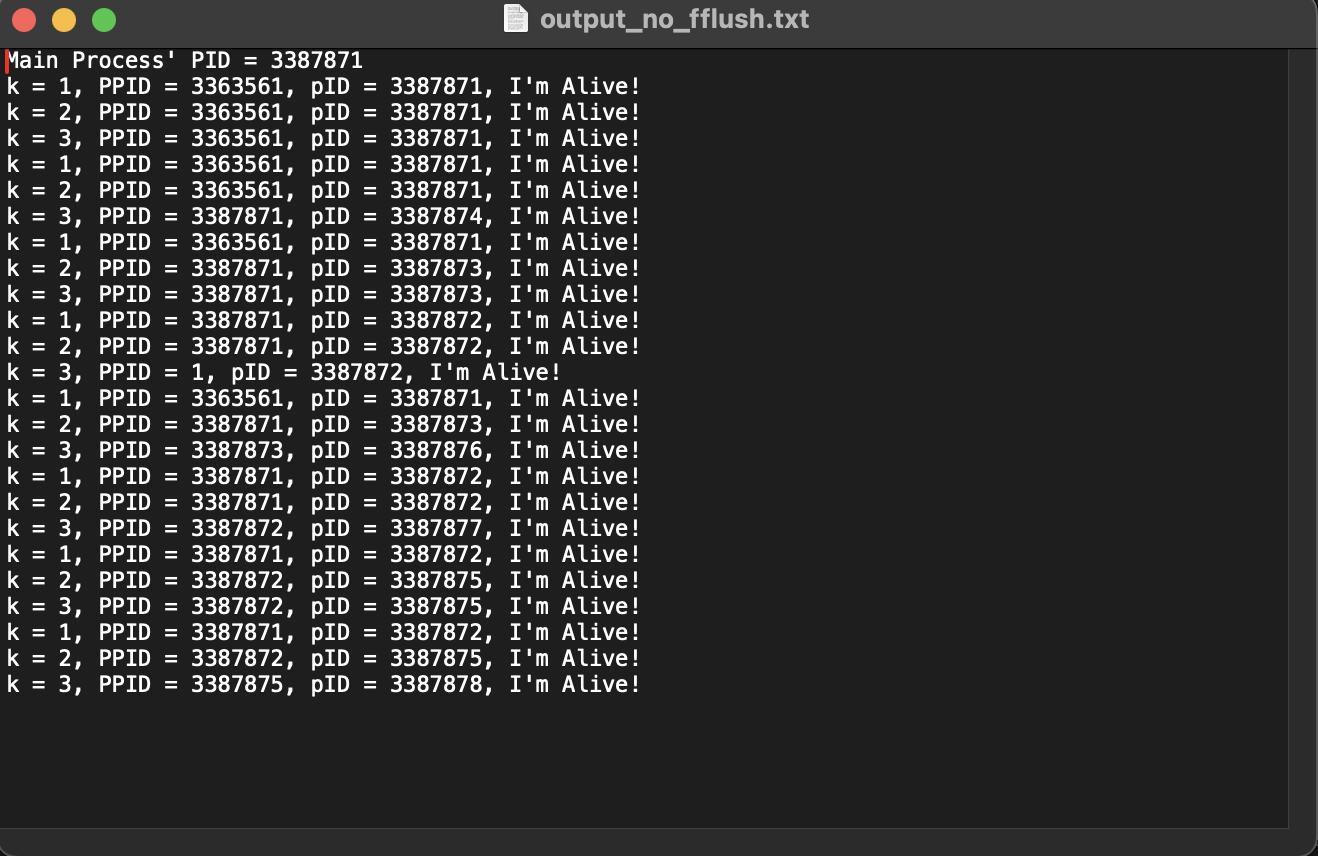
\includegraphics[width=17cm]{output_no_fflush.png}
    \caption{Terminal output when fflush is not used.}
  \end{figure}

\subsection{File Output Analysis}
In output buffering, this compares terminal and file outputs with and without the use of \texttt{fflush}. \texttt{fflush} results in immediate output to the terminal, while without \text{fflush}, the output is buffered, leading to a non-deterministci order in terminal output. Buffered I/O may lead to race conditions. 

\section{Conclusion}
The experiment demonstrates the impact of the fork system call on process creation and management. It also highlights the role of output buffering in the visibility of print statements to the terminal and files.

\vfill
  \section*{Academic Integrity Pledge}
    {\color{red}\textit{“This work complies with the JMU honor code. I did not give or receive unauthorized help on this assignment.”}}

\end{document}
